% Chapter 3

\chapter{Classifier Features and Logical Schema} % Main chapter title

\label{Chapter3} % For referencing the chapter elsewhere, use \ref{Chapter3} 

\lhead{Chapter 3. \emph{Classifier Features}} % This is for the header on each page - perhaps a shortened title

%----------------------------------------------------------------------------------------
%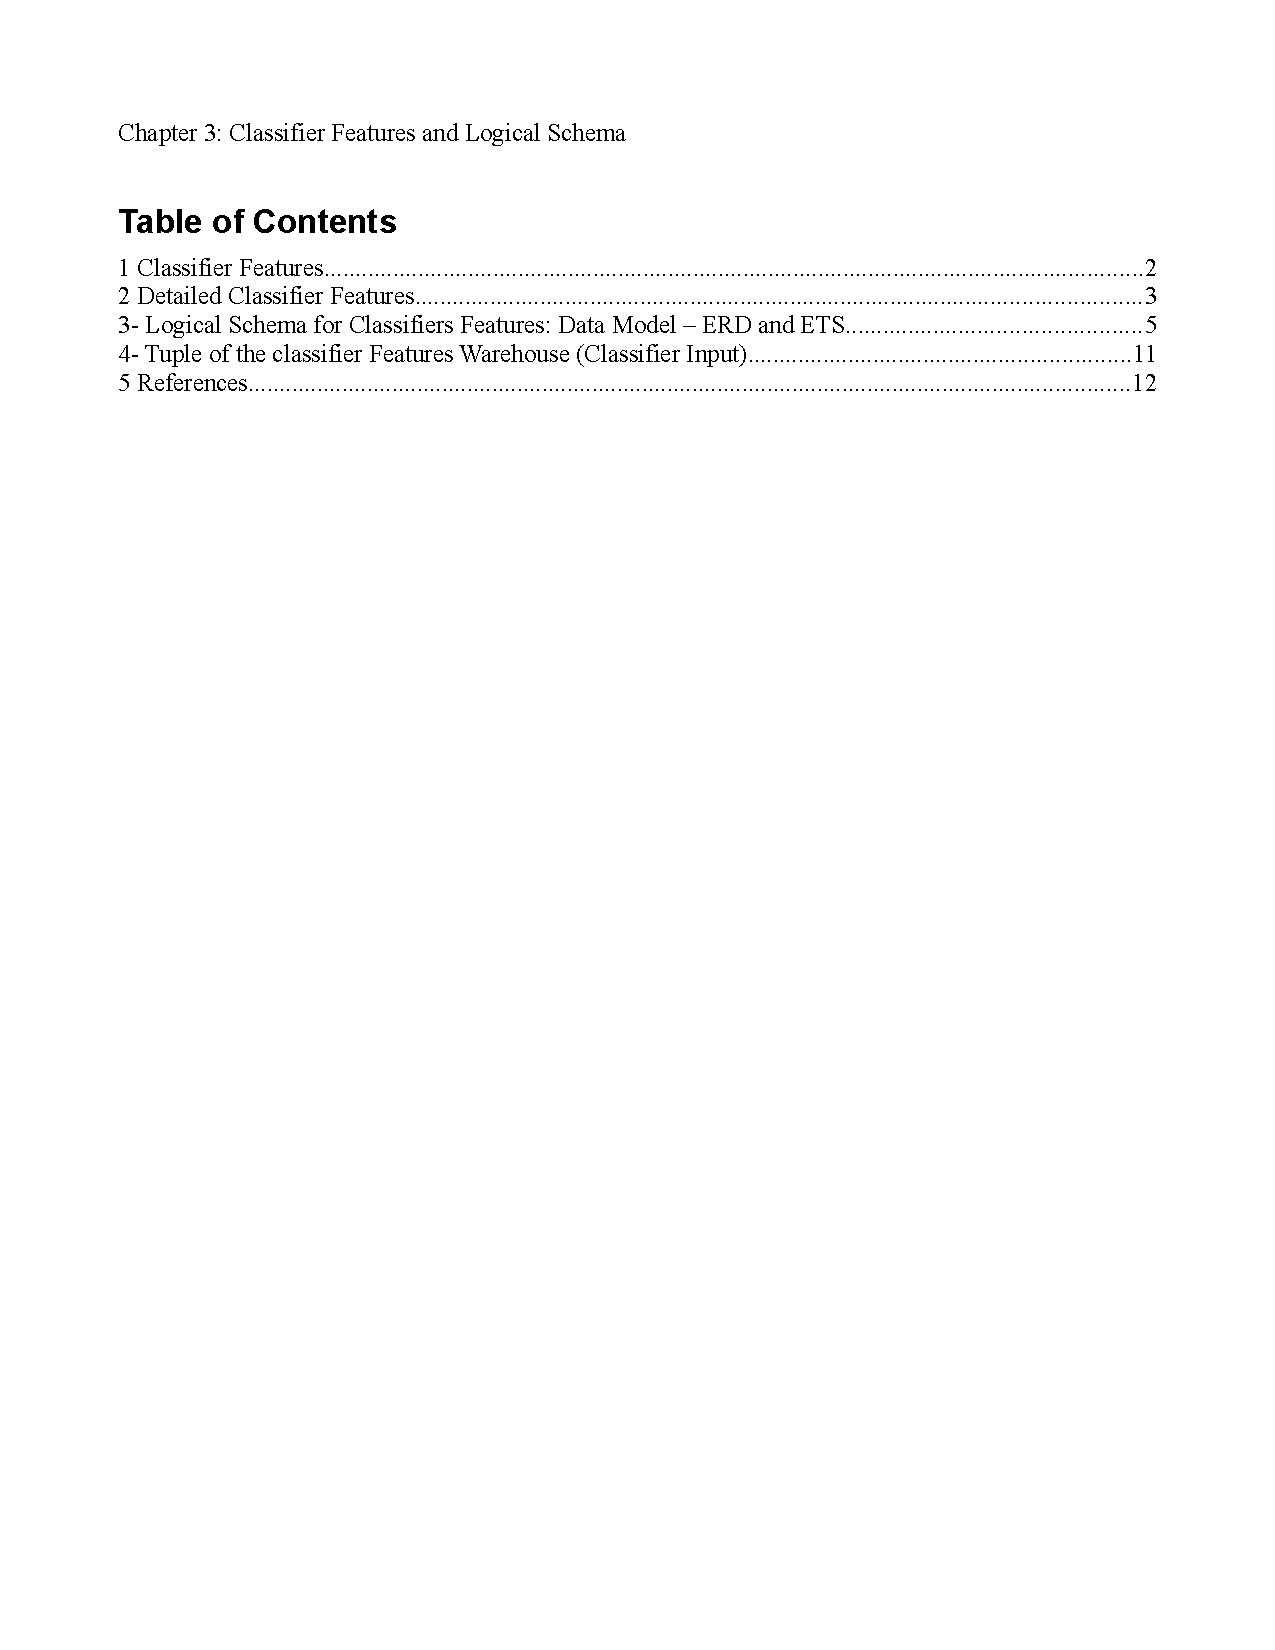
\includepdf[pages=-,offset=14mm 5mm]{Features.pdf}
\section {Classifier Features}
\begin{longtable}{|>{\centering}p{2.5cm}|>{\centering}p{3cm}|>{\centering}p{3cm}|>{\centering}p{3cm}|}
\hline
\multirow{19}{2.5cm}{Features needed for the email classifier (Automatic Categorization
of emails into folders)}
 & \multicolumn{3}{c|}{Features}\tabularnewline
\cline{2-4}
\cline{2-4} 
 & Email & Receiver & Attachment\tabularnewline
\cline{2-4} 
 & Email ID {[}7{]} & Domain of receiver {[}1{]} {[}9{]} &  Attachment  type {[}1{]} {[}9{]}\tabularnewline
\cline{2-4} 
 & Body Length {[}1{]} {[}9{]} & Number of CC {[}1{]} {[}9{]} & Has an attachment {[}1{]} {[}9{]}\tabularnewline
\cline{2-4} 
 & Content Type {[}7{]} & Number of receivers {[}1{]} {[}9{]} & Number of attachments {[}1{]} {[}9{]}\tabularnewline
\cline{2-4} 
 & Domain of sender {[}1{]} {[}9{]} & Number of To {[}1{]} {[}9{]} & \tabularnewline
\cline{2-4} 
 & Email Date {[}3{]} {[}7{]} & Receiver Username {[}1{]} {[}9{]} & \tabularnewline
\cline{2-4} 
 & Email Sender {[}1{]} {[}2{]} {[}7{]} {[}9{]} &  & \tabularnewline
\cline{2-4} 
 & Email Signature {[}9{]} &  & \tabularnewline
\cline{2-4} 
 & Email Subject {[}1{]} {[}2{]} {[}9{]} &  & \tabularnewline
\cline{2-4} 
 & Is Bcc {[}1{]} {[}2{]} {[}9{]} &  & \tabularnewline
\cline{2-4} 
 & Is distribution List {[}1{]} {[}9{]} &  & \tabularnewline
\cline{2-4} 
 & Language {[}1{]} {[}9{]} &  & \tabularnewline
\cline{2-4} 
 & MIME Version {[}7{]} &  & \tabularnewline
\cline{2-4} 
 & Number of punctuation Letters {[}1{]} {[}9{]} &  & \tabularnewline
\cline{2-4} 
 & Percentage of capital letters {[}1{]} {[}9{]} &  & \tabularnewline
\cline{2-4} 
 & Sender Username {[}1{]} {[}9{]} &  & \tabularnewline
\cline{2-4} 
 & Subject Length {[}1{]} {[}9{]} &  & \tabularnewline
\cline{2-4} 
 & Wordgram Frequency {[}1{]} {[}2{]} {[}9{]} &  & \tabularnewline
\hline
\end{longtable}
%----------------------------------------------------------------------
\section {Detailed Classifier Features}

\begin{longtable}{|>{\centering}p{2cm}|>{\centering}p{2.5cm}|>{\centering}p{3cm}|>{\centering}p{3cm}|>{\centering}p{3cm}|}
\hline 
Category & Feature & Description & Values & Source (preparation)\tabularnewline
\hline
\hline 
Email & Email ID {[}7{]} & Identifier for the email message & Long & System maintained primary key\tabularnewline
\hline 
 & Domain of sender {[}1{]} {[}9{]} & Mail Service Provider (gmail.com, hotmail.com, ..etc) & String & Obtained from the sender's email, by taking the substring after the
'@' character\tabularnewline
\hline 
 & Language {[}1{]} {[}9{]} & Dominant language in the email body & String & Use a special module to detect the language type of the email body\tabularnewline
\hline 
 & Email Sender {[}1{]} {[}2{]} {[}7{]} {[}9{]} & Email address of the sender & String & Obtained directly from the email header\tabularnewline
\hline 
 & Content Type {[}7{]} & Content type  & String & Obtained directly from the email header\tabularnewline
\hline 
 & Email Date {[}3{]} {[}7{]} & Date of sending the email represented as the number of milliseconds
since January 1, 1970, 00:00:00 GMT & Long & The date is obtained directly from the email header and then transformed
to the long representation\tabularnewline
\hline 
 & MIME Version {[}7{]} & MIME is an internet standard to extend the format of the email to
support non-ASCII data & Integer & Obtained directly from the email header\tabularnewline
\hline 
 & Bcc {[}1{]} {[}2{]} {[}9{]} & List of email receivers as Bcc & Each recipient is represented as a boolean attribute in the feature
tuple. & Obtained directly from the email header \tabularnewline
\hline 
 & Number of punctuation Letters {[}1{]} {[}9{]} & Number of punctuation characters in the body & Integer & Count the number of punctuation letters in the email body\tabularnewline
\hline 
 & Is distribution List {[}1{]} {[}9{]} & Flag to indicate whether the client received this email from a group/distribution
list or not & Boolean & Obtained directly from email header\tabularnewline
\hline 
 & Email Signature {[}9{]} & Signature of the email sender, at the end of the email & String & The signature is extracted from email body\tabularnewline
\hline 
 & Wordgram Frequency {[}1{]} {[}2{]} {[}9{]} & Email Wordgram Frequency & Integer & Count the number of wordgrams in the email\tabularnewline
\hline 
 & Subject Length {[}1{]} {[}9{]} & Length of the email subject & Integer & Calculate the size of the subject string\tabularnewline
\hline 
 & Percentage of capital letters {[}1{]} {[}9{]} & Percentage of the capital letters to the letters in the email body & Double & Count the number of capital letters and divide it by the sum of the
sizes of all ASCII words in the email body\tabularnewline
\hline 
 & Body Length {[}1{]} {[}9{]} & Size of the email body & Integer & Calculate the size of the body string\tabularnewline
\hline 
 & Sender Username {[}1{]} {[}9{]} & Name of Sender & String & Obtained directly from email header\tabularnewline
\hline 
 & Total Number of words & Number of words in the email body & Integer & Calculate the number of words in the email body\tabularnewline
\hline 
 & Email Subject {[}1{]} {[}2{]} {[}9{]} & Subject of the email & String & Obtained directly from the email header\tabularnewline
\hline 
Receiver & Receiver Username {[}1{]} {[}9{]} & Name of receiver & String & Obtained directly from email header\tabularnewline
\hline 
 & Number of receivers {[}1{]} {[}9{]} & Number of email receivers & Integer & Count the number of receivers obtained from email header\tabularnewline
\hline 
 & Number of CC {[}1{]} {[}9{]} & Number of CC recipients & Integer & Count the number of CC recipients obtained from email header\tabularnewline
\hline 
 & Number of To {[}1{]} {[}9{]} & Number of CC & Integer & Count the number of receivers mentioned in the TO header\tabularnewline
\hline 
 & Domain of receiver {[}1{]} {[}9{]} & Mail Service Provider(s) for the receiver(s) & String & Obtained directly from email header\tabularnewline
\hline 
Attachment & Number of attachments {[}1{]} {[}9{]} & Number of attached files in the email  & Integer & Count the number of attachments obtained from the IMAP interface\tabularnewline
\hline 
 &  Attachment  type {[}1{]} {[}9{]} & Type of attachment & String & 	Has an attachment {[}1{]} {[}9{]}	Flag to denote whether the email
has an attachment	Boolean 	If the number of attachment is zero, return
false, else return true
\tabularnewline
\hline
\end{longtable}
%----------------------------------------------------------------------
\section{Logical Schema for Classifiers Features: Data Model – ERD and ETS}
Illustration 1: Logical Conceptual View of the classifier features Data Model (DM)
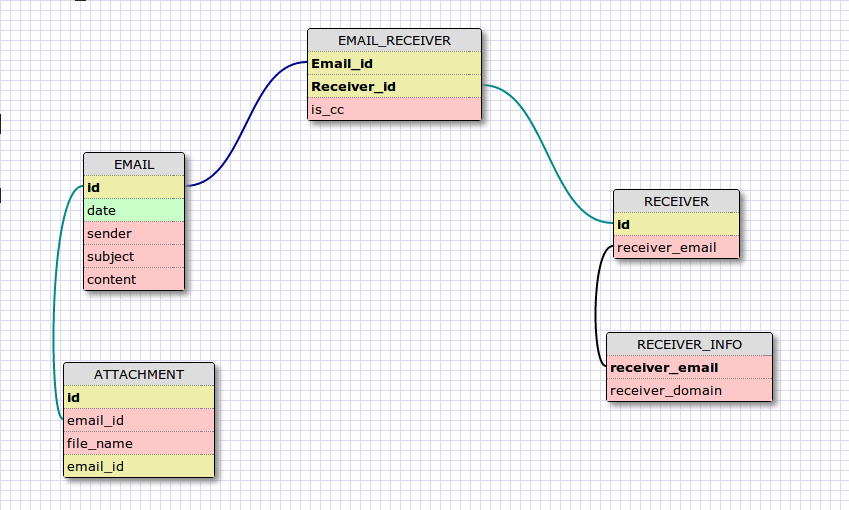
\includegraphics[scale=0.5]{erd1.png}
\\

Illustration 2: Mapping DM into Entity Relationship Diagram (ERD)
\\
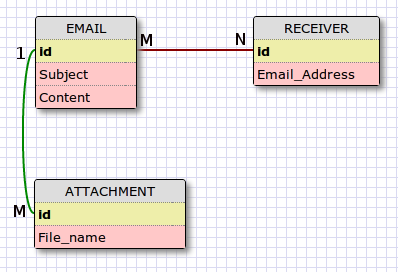
\includegraphics[scale=0.7]{erd2.png}
\newpage

\begin{tabular}{|>{\centering}p{3cm}|>{\centering}p{3cm}|>{\centering}p{2.5cm}|>{\centering}p{3cm}|}
\hline 
\textbf{Project}: \underbar{Smart Email } & \textbf{Subject}: \underbar{Classifier Features} & \multicolumn{2}{>{\centering}p{5.5cm}|}{\textbf{Page}: 1/1}\tabularnewline
\hline
\hline 
\textbf{Entity}: \underbar{Email}  & \textbf{Date}: \underbar{Thursday,}

\underbar{March 1,2012} & \multicolumn{2}{>{\centering}p{5.5cm}|}{\textbf{Analyst}:}\tabularnewline
\hline 
\textbf{Attribute } & \textbf{Type} & \textbf{Size} & \textbf{Validation / desc}\tabularnewline
\hline 
Id  & Integer & 4 Bytes & Primary Key, system maintained,used to identify emails\tabularnewline
\hline 
date & Date & - & the date the email was received in\tabularnewline
\hline 
sender & String & 40 Characters & The email address of the email sender\tabularnewline
\hline 
subject & String & 40 Characters & The Subject of the email\tabularnewline
\hline 
content & Text & - & The body of the email\tabularnewline
\hline
\end{tabular}

\newpage

\begin{tabular}{|>{\centering}p{3cm}|>{\centering}p{3cm}|>{\centering}p{2.5cm}|>{\centering}p{3cm}|}
\hline 
\textbf{Project}: \underbar{Smart Email} & \textbf{Subject}: \underbar{Classifier Features} & \multicolumn{2}{>{\centering}p{5.5cm}|}{\textbf{Page}: 1/1}\tabularnewline
\hline
\hline 
\textbf{Entity}: \underbar{ATTACHMENT} & \textbf{Date}: \underbar{Thursday,}

\underbar{March 1, 2012} & \multicolumn{2}{>{\centering}p{5.5cm}|}{\textbf{Analyst}:}\tabularnewline
\hline 
\textbf{Attribute} & \textbf{Type} & \textbf{Size} & \textbf{Validation / desc}\tabularnewline
\hline 
Id & Integer & 4 Bytes & Primary Key, system maintained, used to identify different attachments\tabularnewline
\hline 
email\_id & Integer & 4 Bytes & Foreign key to EMAIL.id\tabularnewline
\hline 
file\_name & String & 40 Characters & Name of the attachment\tabularnewline
\hline
\end{tabular}

\newpage

\begin{tabular}{|>{\centering}p{3cm}|>{\centering}p{3cm}|>{\centering}p{2.5cm}|>{\centering}p{3cm}|}
\hline 
\textbf{Project}: \underbar{Smart Email} & \textbf{Subject}: \underbar{Classifier Features} & \multicolumn{2}{>{\centering}p{5.5cm}|}{\textbf{Page}: 1/1}\tabularnewline
\hline
\hline 
\textbf{Entity}: \underbar{RECEIVER} & \textbf{Date}: \underbar{Thursday,}

\underbar{March 1, 2012} & \multicolumn{2}{>{\centering}p{5.5cm}|}{\textbf{Analyst}:}\tabularnewline
\hline 
\textbf{Attribute} & \textbf{Type} & \textbf{Size} & \textbf{Validation / desc}\tabularnewline
\hline 
Id & Integer & 4 Bytes & Primary Key, system maintained, used to identify different recipients\tabularnewline
\hline 
receiver\_email & String & 40 Characters & Email of the receiver\tabularnewline
\hline 
receiver\_name & String & 40 Characters & Name of the receiver\tabularnewline
\hline 
receiver\_domain & String & 40 Characters & Domain of the receiver\tabularnewline
\hline
\end{tabular}

\newpage


\begin{tabular}{|>{\centering}p{3.2cm}|>{\centering}p{3cm}|>{\centering}p{2.5cm}|>{\centering}p{3cm}|}
\hline 
\textbf{Project}: \underbar{Smart Email} & \textbf{Subject}: \underbar{Classifier Features} & \multicolumn{2}{>{\centering}p{5.5cm}|}{\textbf{Page}: 1/1}\tabularnewline
\hline
\hline 
\textbf{Entity}:

\underbar{EMAIL\_RECEIV}

\underbar{ER} & \textbf{Date}: \underbar{Thursday,}

\underbar{March 1, 2012} & \multicolumn{2}{>{\centering}p{5.5cm}|}{\textbf{Analyst}:}\tabularnewline
\hline 
\textbf{Attribute} & \textbf{Type} & \textbf{Size} & \textbf{Validation / desc}\tabularnewline
\hline 
email\_id & Integer & 4 Bytes & Composite Primary Key, system maintained, used to identify different
email/receiver tuple\tabularnewline
\cline{1-3} 
receiver\_id & Integer & 4 Byte & \tabularnewline
\hline 
is\_cc & Boolean & 1 Byte & Used to indicate whether this receiver is mentioned in cc header or
not\tabularnewline
\hline

\end{tabular}

%-------------------------------------------------------------------------
\newpage
\section {Tuple of the classifier Features Warehouse (Classifier Input)}

\begin{center}
\begin{tabular}{|c|}
\hline 
email\_id\tabularnewline
\hline
date\tabularnewline
\hline 
sender\_email\tabularnewline
\hline 
sender\_username\tabularnewline
\hline 
Domain of sender\tabularnewline
\hline 
is\_bbc\tabularnewline
\hline 
subject\tabularnewline
\hline 
Subject\_length\tabularnewline
\hline 
content\tabularnewline
\hline 
content\_mime\_version\tabularnewline
\hline 
body\_length\tabularnewline
\hline 
signature\tabularnewline
\hline 
number\_of\_receivers\tabularnewline
\hline 
Percentage\_of\_capital\_letters\tabularnewline
\hline 
Number\_of\_punctuation\_letters\tabularnewline
\hline 
language\tabularnewline
\hline 
has\_attachments\tabularnewline
\hline 
number\_of\_attachments\tabularnewline
\hline
\end{tabular}
\end{center}

\newpage




\begin{tabular}{|>{\centering}p{3.2cm}|>{\centering}p{3cm}|>{\centering}p{2.5cm}|>{\centering}p{4.5cm}|}
\hline 
\textbf{Project}: \underbar{Smart Email} & \textbf{Subject}: \underbar{Classifier Features} & \multicolumn{2}{>{\centering}p{7cm}|}{\textbf{Page}: 1/2}\tabularnewline
\hline
\hline 
\textbf{Entity}: \underbar{Feature\_tuple} & \textbf{Date}: \underbar{Thursday,}

\underbar{March 1, 2012} & \multicolumn{2}{>{\centering}p{7cm}|}{\textbf{Analyst}:}\tabularnewline
\hline 
\textbf{Attribute} & \textbf{Type} & \textbf{Size} & \textbf{Validation / desc}\tabularnewline
\hline 
Id & Integer & 4 Bytes & Primary Key, system maintained, used to identify different feature\_tuples\tabularnewline
\hline 
email\_id & Integer & 4 Bytes & Foreign key to EMAIL.Id\tabularnewline
\hline 
date & Date & - & Date of sending the email in the long representation\tabularnewline
\hline 
sender\_email & String & 40 Characters & Email of the sender\tabularnewline
\hline 
sender\_user\_name & String & 40 Characters & Name of the sender as it appears in the contacts list\tabularnewline
\hline 
domain\_of\_sender & String & 40 Characters & Email Service Provider for the sender\tabularnewline
\hline 
 is\_bcc & Boolean & 1 Byte & Indicates whether the user received this email as a recipient or as
a Bcc recipient\tabularnewline
\hline 
subject & String & 40 Characters & The Subject of the email\tabularnewline
\hline 
subject\_length & Integer & 4 Bytes & Length of the email subject\tabularnewline
\hline 
content & Text & - & Email body\tabularnewline
\hline 
content\_type & String & 40 Characters & Content type of the email\tabularnewline
\hline 
content\_mime\_

version & Integer & 4 Bytes & MIME version of the email\tabularnewline
\hline 
body\_length & Integer & 4 Bytes & Length of the email body\tabularnewline
\hline 
signature & String & 512 Characters & Sender's signature at the end of the email message\tabularnewline
\hline 
number\_of\_attac

hments & Integer & 4 Bytes & Number of attachments in the email\tabularnewline
\hline


\end{tabular}

\newpage


\begin{tabular}{|>{\centering}p{3.2cm}|>{\centering}p{3cm}|>{\centering}p{2.5cm}|>{\centering}p{4.5cm}|}
\hline 
\textbf{Project}: Smart \underbar{Email} & \textbf{Subject}: \underbar{Classifier Features} & \multicolumn{2}{>{\centering}p{7cm}|}{\textbf{Page}: 2/2}\tabularnewline
\hline
\hline 
\textbf{Entity}: \underbar{Feature\_tuple} & \textbf{Date}: \underbar{Thursday,}

\underbar{March 1, 2012} & \multicolumn{2}{>{\centering}p{7cm}|}{\textbf{Analyst}:}\tabularnewline
\hline 
\textbf{Attribute} & \textbf{Type} & \textbf{Size} & \textbf{Validation / desc}\tabularnewline
\hline 
number\_of\_recei

vers & Integer & 4 Bytes & Number of email recipients\tabularnewline
\hline 
percentage\_of\_c

apital\_letters & Double & 8 Bytes & Percentage of capital letters in the email body\tabularnewline
\hline 
number\_of\_punc

tuation & Integer & 4 Bytes & Number of punctuation letters in the email body\tabularnewline
\hline 
language & String & 40 Characters & Dominant language of the email body\tabularnewline
\hline 
has\_attachments & Boolean & 1 Byte & True if the email has attachments, false otherwise\tabularnewline
\hline
\end{tabular}
%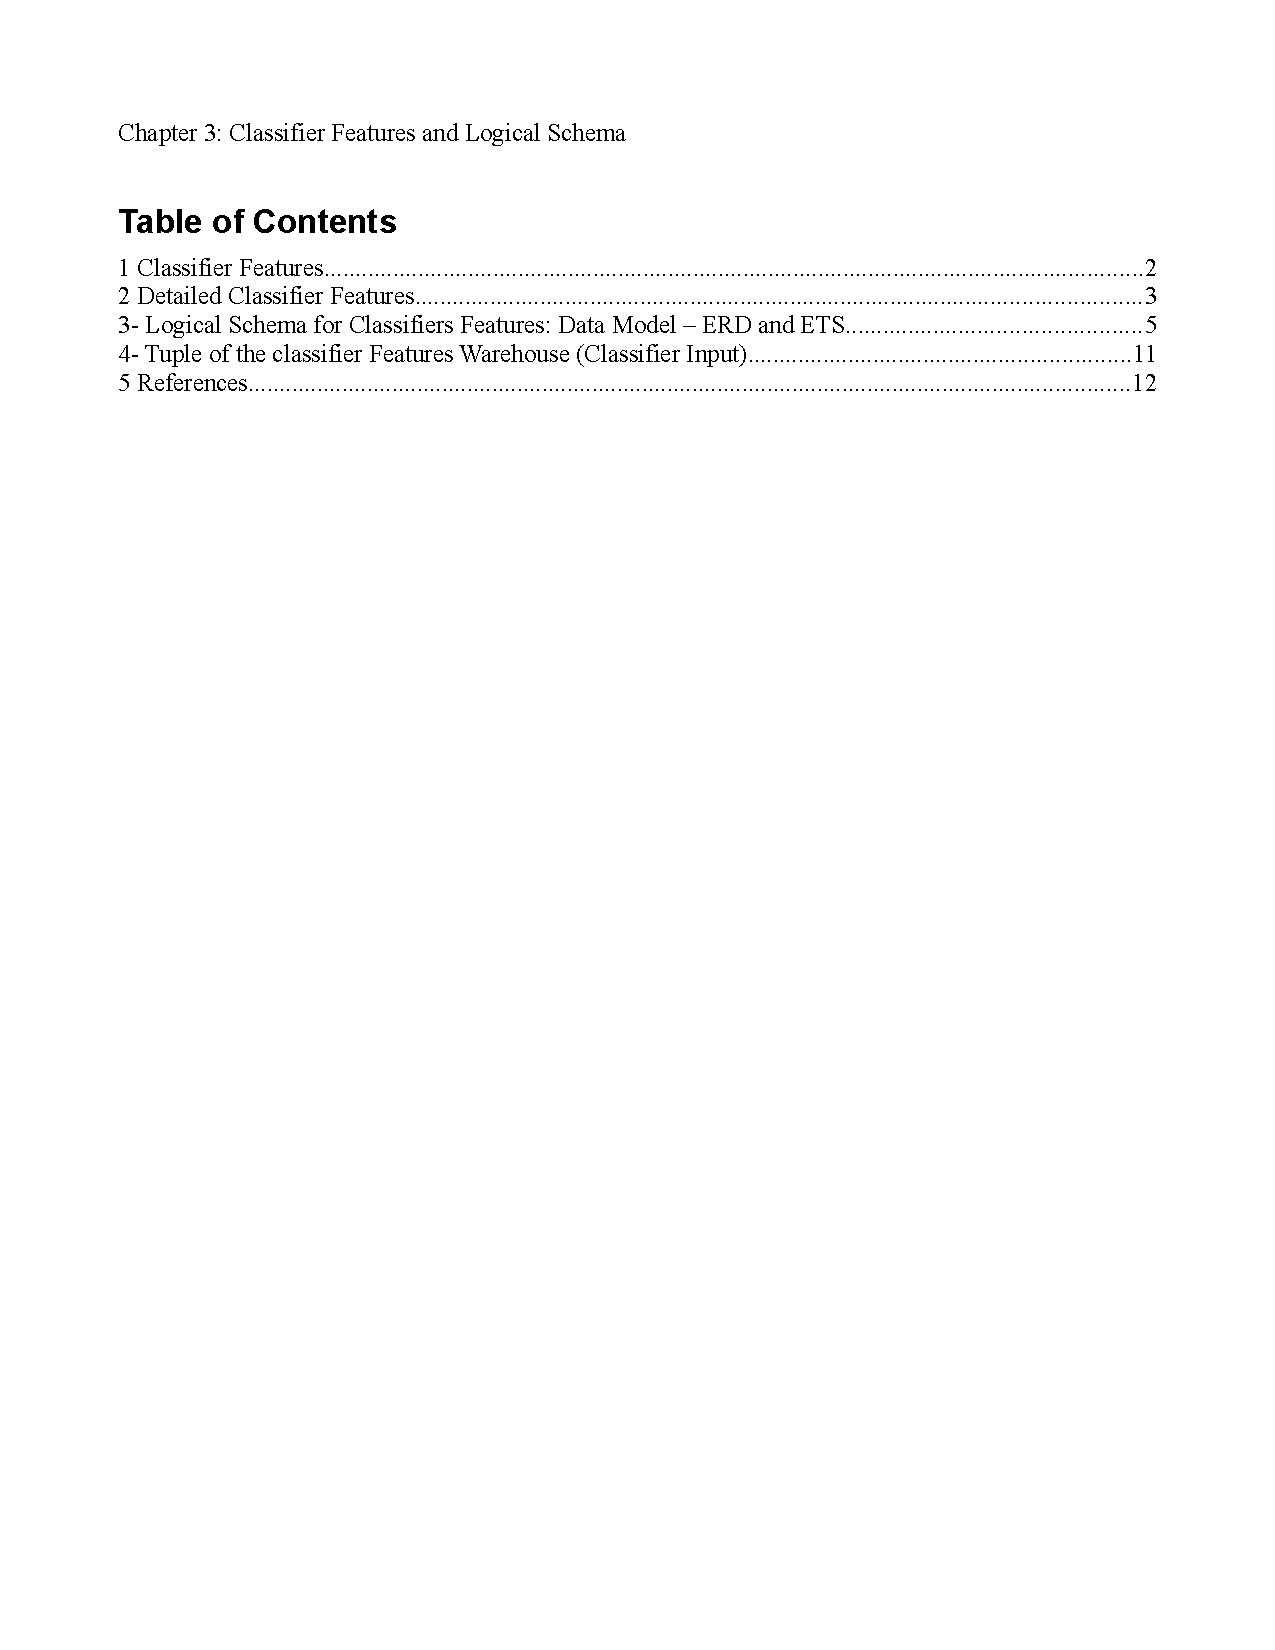
\includegraphics{Features.pdf}\\
